\chapter{Bonus: A Search for Milli-Charged Particles at the LHC}
{\small

\section{Motivation of a search for milli-charged particles}

One of the central mysteries of modern particle physics is the question of what
makes up dark matter. It must consist of massive particles that interact
at most very weakly with the SM, and no viable candidate exists among the
currently known particles. Moreover, a decade's worth of data from the LHC
has provided no evidence of any new particles that might provide an explanation.

We thus ask the question, what types of signatures might hypothetical dark matter
particles produce that would escape detection at present experiments?
One method of explaining dark matter is to add a new ``dark sector'' of
particles beyond the SM that couples only weakly to the SM. As an example,
we can add a ``dark photon'' $A'_\mu$ and a ``dark fermion'' $\psi'$ charged
under the new gauge field with charge $e'$. Allowing for kinetic
mixing between $A'_\mu$ and the SM weak hypercharge field $B_\mu$, the Lagrangian
for this new dark sector can be written
\be\label{eq:mcp_lagr}
\begin{split}
\mathcal{L}_\text{dark-sector} = &-\frac{1}{4}A'_{\mu\nu}A'^{\mu\nu} \\
&+i\bar{\psi}'(\gamma^\mu\partial_\mu + ie'\gamma^\mu A'_\mu + iM_\text{mCP})\psi' \\
&-\frac{\kappa}{2}A'_{\mu\nu}B^{\mu\nu},
\end{split}
\ee
where the first line is the kinetic term for a massless dark photon,
the second line contains the kinetic terms for a dark fermion with
mass $M_\mrm{mCP}$ as well as the interaction term with $A'_\mu$, and
the third line contains the mixing term between $A'_\mu$ and $B_\mu$, with
mixing strength parameter $\kappa$.

The mixing term can be eliminated by redefining $A'_{\mu\nu}\to A'_{\mu\nu}+\kappa B_{\mu\nu}$,
resulting in an interaction term $\kappa e'\bar{\psi}'\gamma^\mu B_\mu\psi$ between $\psi'$
and $B_\mu$. Rewriting $B_\mu$ in terms of the physical photon and $Z$ boson fields
as $B_\mu=\cos\theta_w A_\mu - \sin\theta_w Z_\mu$, we find that the new dark fermion
couples to the SM photon with electric charge $\kappa e'\cos\theta_w$, and couples to the 
SM $Z$ with charge $\kappa e'\sin\theta_w$. The mixing strength $\kappa$ must be small
(otherwise the new dark sector would have been observed already), so we must have
$\varepsilon\equiv \kappa e'\cos\theta_w \ll 1$, and we call $\psi'$ a
``milli-charged particle'' (mCP; note that the name is a bit of a misnomer because $\varepsilon$
does not have to be exactly $\mathcal{O}10^{-3}$))

\begin{figure}[t]
  \begin{center}
    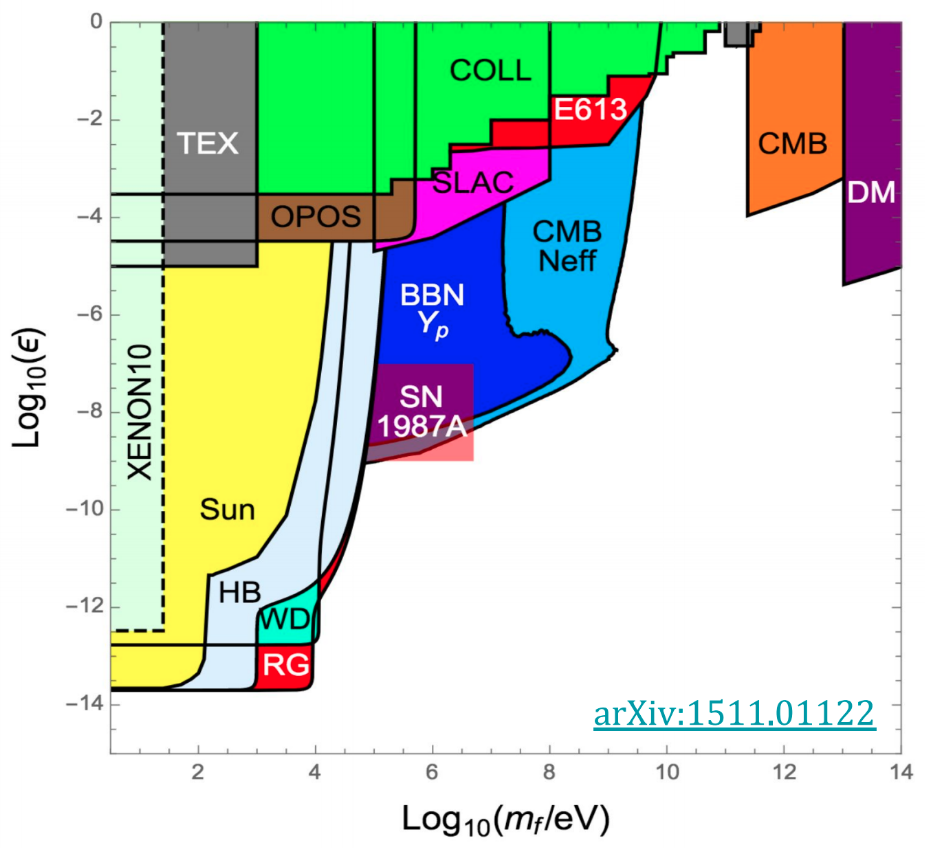
\includegraphics[width=0.50\textwidth]{figs/milliq/search_status.png}
    \caption{Existing exclusion limits for milli-charged partcles, coming
      from searches via colliders, solar effects, astronomical observations,
      and cosmological bounds. milliQan targets the unexcluded phase space
      with $\varepsilon\geq10^{-3}$ and $10^{-1} < m_\text{mCP} < 10^2\GeV$.
      (Image from~\cite{Vinyoles:mcp})
            }
    \label{fig:mcp_search_status}
  \end{center}
\end{figure}

Such milli-charged particles have been searched for via a variety of methods,
either directly through collider experiments or indirectly through
solar effects, astronomical observations, or cosmological bounds.
A summary of the present exclusion space in the mCP mass--charge plane
is shown in Fig.~\ref{fig:mcp_search_status}, taken from~\cite{Vinyoles:mcp}.

There is a gap in the excluded phase space for $\varepsilon>10^{-3}$ at
the mass scales relevant at the LHC, roughly $10^{-1} < m_\text{mCP} < 10^2\GeV$.
mCPs at such masses and charges would be produced frequently at the LHC, but
present experiments would not be able to detect them; direct sensitvity is lost
for $\varepsilon$ below a few times $10^{-1}$, and a low cross section
precludes missing energy searches. Therefore, a dedicated experiment is necessary
to search for mCPs at the LHC.


\section{Overview of the milliQan detector}
The milliQan experiment, designed to search for mCPs using collisions at LHC P5, was proposed in 
2015~\cite{Haas:mcp,mq:loi}. It is located in a drainage gallery, elevated 45$^\circ$ above and 33
m from the CMS experiment, with 17 m of rock in between that naturally
suppresses beam-based backgrounds. The proposed design consists of three stacked layers of plastic 
scintillator arrays, with each scintillating bar coupled to a photomultiplier tube (PMT).
The arrays are pointed at the interaction point (IP), such that a particle originating
from a $pp$ collision would pass through all three layers in a straight line.
The bars are sensitive enough to detect individual photoelectrons produced by
throughgoing mCPs, and requiring a simultaneous hit in all three layers drastically
reduces background, which mostly consists of random overlap of pulses from
PMT dark rate, environmental radiation, cosmic rays, and afterpulsing.

The full milliQan design is anticipated to consist of three ``layers'' of $20\times20$ scintillator arrays,
each around 1 m$^2$ in total. In 2017--18, a smaller scale \textit{demonstrator} was installed
to study backgrounds and provide a proof-of-concept for the full-scale detector.
This demonstrator consists of three $2\times3$ scintillator bar arrays, roughly 1--2\%
of the planned full detector.

The 18 scintillator bars each measure 5 cm $\times$ 5 cm $\times$ 80 cm, and are
wrapped in layers of reflective and light-blocking materials to ensure optimal
efficiency. 3D-printed plastic casings couple the bars to individual PMTs
(two Hamamatsu R7725s, four Electron Tube 9814Bs, and 12 Hamamatsu R878s).

\begin{figure}[t]
  \begin{center}
    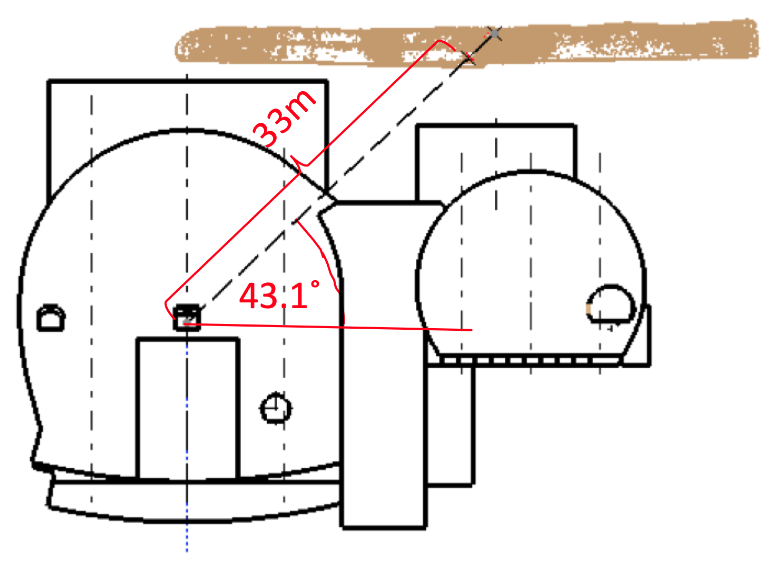
\includegraphics[width=0.440\textwidth]{figs/milliq/cavern_loc.png}
    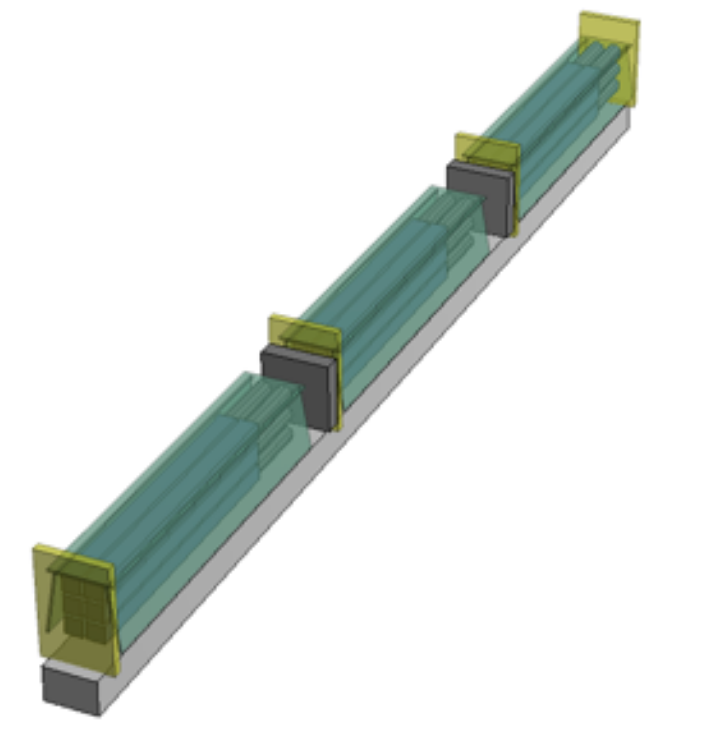
\includegraphics[width=0.352\textwidth]{figs/milliq/demonstrator_illustration.png}
    \caption{(left) Illustration of the location of the drainage gallery with 
      respect to the CMS cavern. CMS is located in the large dome on the left; 
      milliQan is elevated 43.1$^\circ$ above this, and 33 m away, with 17 m of
      rock in between. (right) 3D illustration of the demonstrator detector.
      The slabs are in yellow, the panels in translucent green, and the bars can be seen through
      the panels. The gray blocks in the layer gaps are lead bricks to block radiation.
            }
    \label{fig:demonstrator}
  \end{center}
\end{figure}

In addition to the scintillator bars, there are four 20 cm $\times$ 30 cm $\times$ 2.5 cm
scintillator ``slabs'' placed at the front and rear of the detector
as well as in between the layers, in order to tag/veto beam-based and cosmic
particles. Additionally, each layer has three 18 cm $\times$ 102 cm $\times$ 0.7 cm scintillator
``panels'' covering the top and sides, in order to tag/veto cosmic particles and environmental radiation.
Each of the slabs and panels is read out by a Hamamatsu R878 PMT.

There are 5 cm-thick lead bricks placed between each layer to reduce correlated pulses from radiation.
All of the scintillators and lead bricks are mounted on a custom-designed aluminum support structure
that can rotate the entire stack in multiple directions to facilitate alignment with the IP.
A CERN engineering team performed such an alignment, so that the detector points
to the IP to within a tolerance of just 1 cm over the 33 m distance. The location of the drainage gallery
and an illustration of the demonstrator are shown in Fig.~\ref{fig:demonstrator}.

The 31 scintillator channels are read out by a pair of CAEN V1743 digitizers, which sample at 1.6 GHz
and record a 640 ns waveform for each channel upon triggering. The trigger can be configured
to fire on single, double, or triple coincidence of peaks at an arbitrary threshold.
For nominal data taking, the trigger is set to fire on a triple coincidence of pulses.

\section{Bench tests for PMT calibration}
\label{sec:pmt_bench_tests}

The demonstrator detector makes use of three different ``species'' of PMTs, each of which
has very different characteristics. Even PMTs within the same species differ somewhat
in their behavior. It is therefore necessary to calibrate each PMT individually, so
that data can be interpreted correctly and simulation can be adjusted to accurately
model the behavior of the real detector.

Two separate calibrations are necessary. The first is the efficiency of the PMT
to convert an optical photon into a photoelectron (PE). Once installed in the detector, 
this is intertwined with the efficiency of the scintillators themselves to generate
and propagate the photons, so it is measured ``in-situ'', and described in the following
section. The other calibration involves the response of the PMT to a single photoelectron (SPE),
which includes the pulse shape and pulse area distribution. The mean pulse area
is also measured in-situ, as it can be affected by small magnetic fields and other effects,
but we perform measurements of the pulse shapes and full area distributions in the lab
using flashing LEDs, in order to (1) cross-check the in-situ measurements
and (2) generate the necessary inputs for the pulse-injection step of the simulation,
described in Sec.~\ref{sec:mq_mcgen}.

For the LED bench tests, we largely follow the method outlined in~\cite{Saldanha:pmt},
which allows for the measurement of the non-Gaussian low-area
tails of the SPE area distributions, arising from non-optimal trajectories
within the PMT (e.g. the photon skipping the cathode and directly hitting
the first dynode, or a photoelectron skipping a dynode stage).
The laboratory setup is sketched in Fig.~\ref{fig:pmt_setup}.
A blue LED and a PMT are placed in a light-tight enclosure,
and the LED is flashed in short $\sim$10 ns bursts so that the PMT
generates $\mathcal{O}(1)$ PE on average. The PMT is read out with
a DRS board~\cite{drs}, which is triggered on the LED pulse
so that even 0 PE events are recorded. An optional cardboard light-blocker
can be inserted between the LED and PMT, to collect a pure sample of 0 PE events.

\begin{figure}[t]
  \begin{center}
    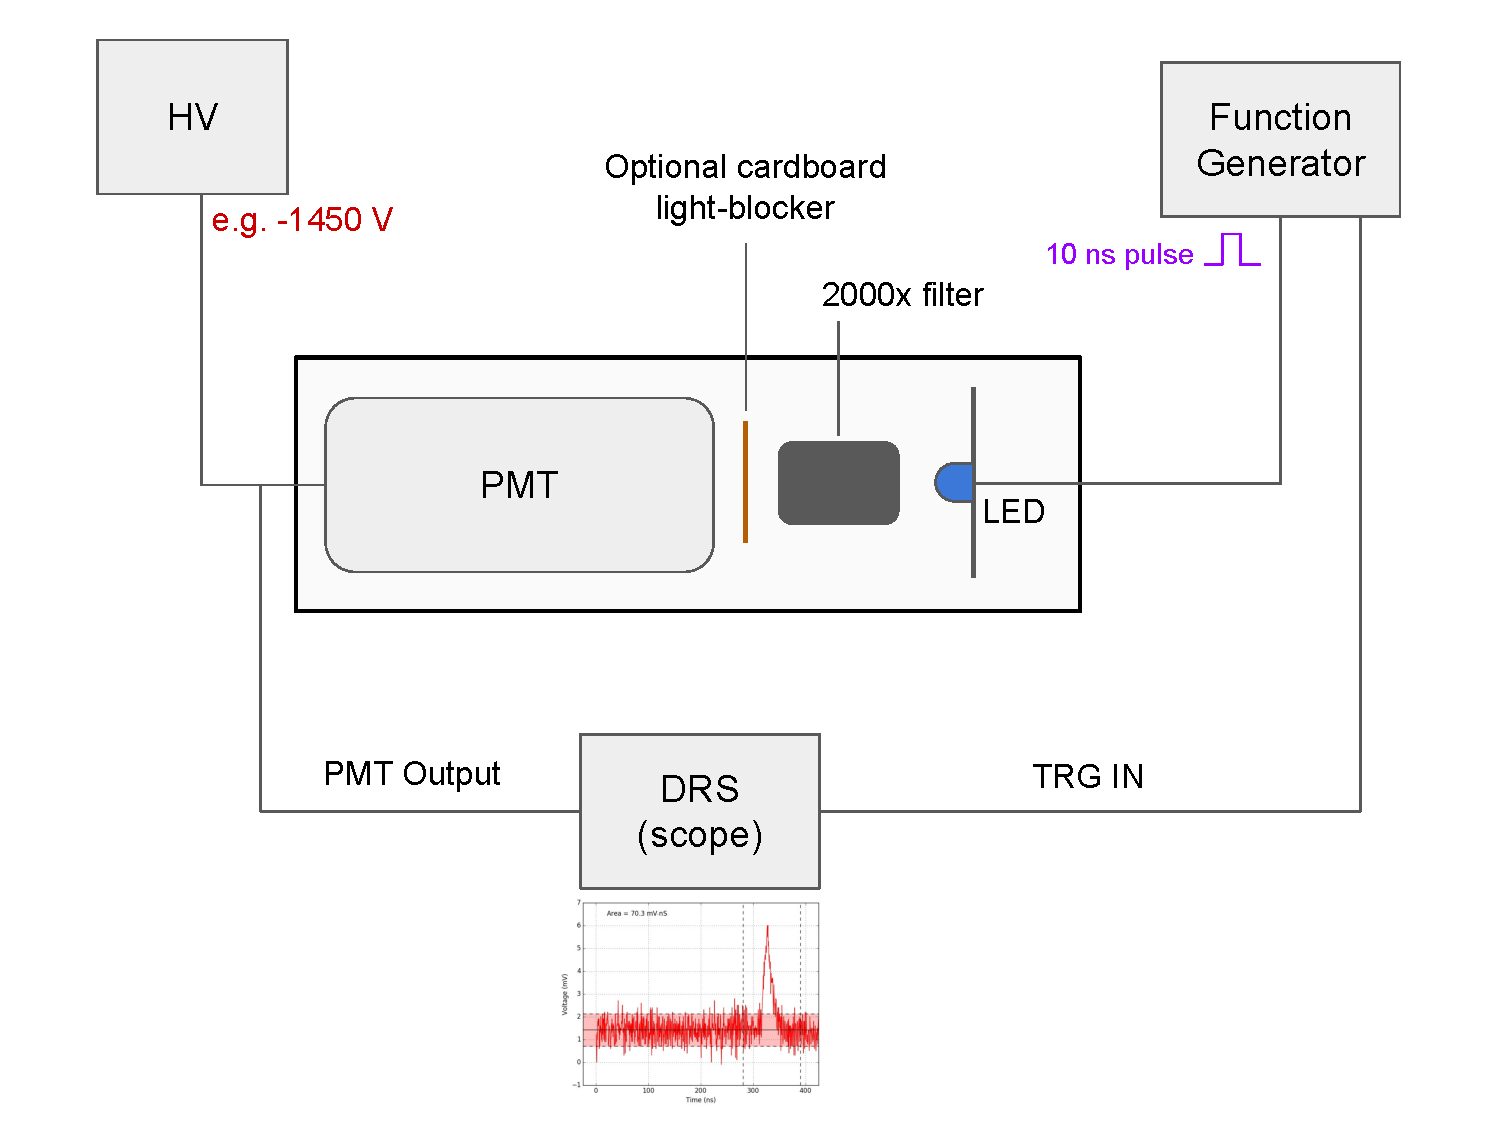
\includegraphics[width=0.750\textwidth]{figs/milliq/pmt_setup.pdf}
    \caption{Diagram of the laboratory setup for LED bench tests of the PMTs.
      An LED and the PMT are mounted in a light-tight 3D-printed casing,
      with a 2000x optical filter in between. The LED is flashed in
      short $\sim$10 ns pulses, and the PMT signal is read out by
      a DRS evaluation board~\cite{drs}. The board is triggered not by the 
      PMT but by the LED pulse generator, so that even ``blank'' (0 PE) events
      are recorded. An optional cardboard light-blocker can be inserted between
      the LED and PMT, in order to collect a pure sample of 0 PE events.
            }
    \label{fig:pmt_setup}
  \end{center}
\end{figure}

Upon each LED pulse, the PMT waveform is recorded. The pulse (when there is $\geq1$ PE)
occurs at the same time in each event, so there is no peak-finding necessary and the 
area can be computed by integrating over a fixed time window. Doing this for many
events, one can build up a histogram of pulse areas, and if the LED intensity is
set correctly one can observed distinct peaks in the distribution corresponding
to 0, 1, 2,$\dots$ PE events. Fig.~\ref{fig:led_events} shows an example
R878 waveform and the pulse area distributions for a few different 
high-voltages (HVs).

\begin{figure}[t]
  \begin{center}
    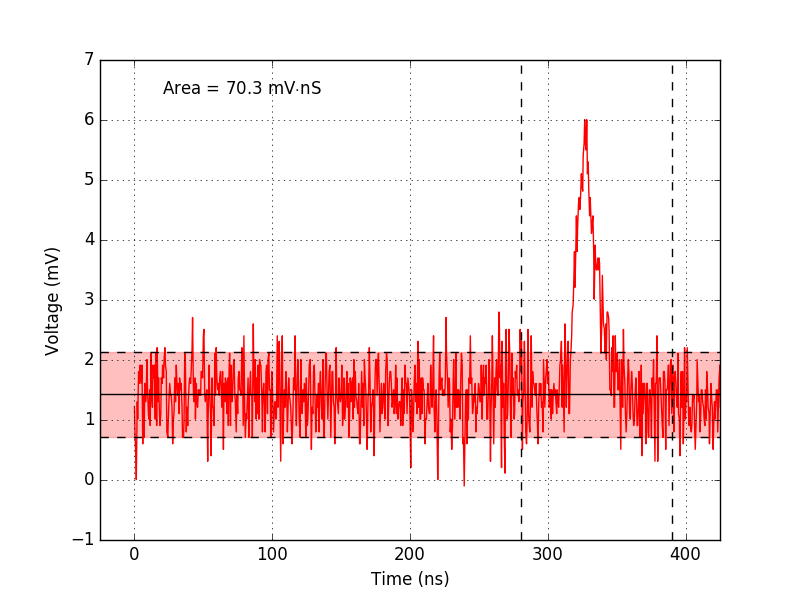
\includegraphics[width=0.450\textwidth]{figs/milliq/example_led_event_878.png}
    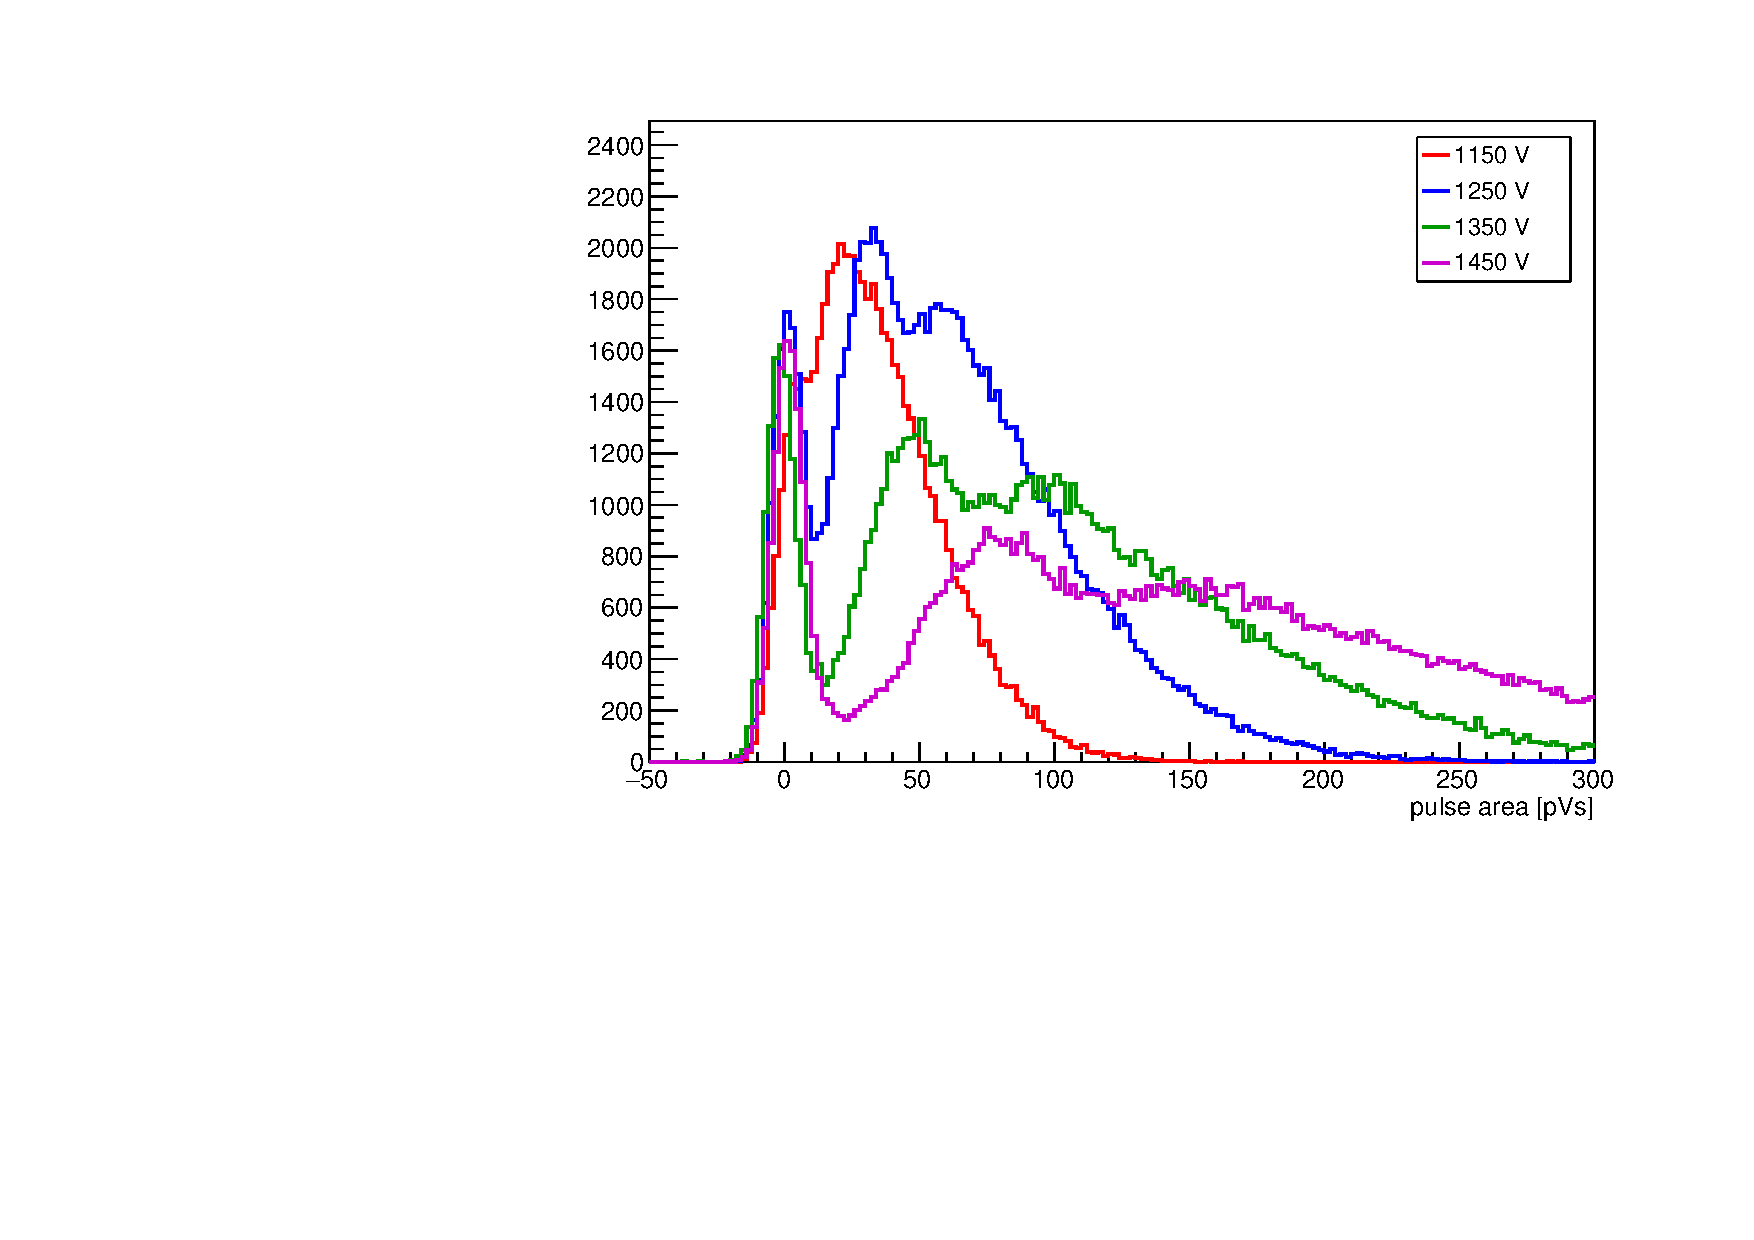
\includegraphics[width=0.500\textwidth]{figs/milliq/pmt_areas_hv_scan.pdf}
    \caption{(left) An example SPE waveform and (right) the pulse area distributions
      for a variety of HVs, for an R878 PMT. The LED intensity is set so that
      the 
            }
    \label{fig:led_events}
  \end{center}
\end{figure}

The calibration method makes use of the fact that the number of observed photoelectrons
after the LED light is heavily filtered is a Poisson process. Two datasets are recorded:
one with no cardboard light-blocker, and the LED intensity set so that there
is $\mathcal{O}(1)$ PE on average per event, and one with the light-blocker inserted
(but with the LED running at the same intensity, so that any electronic effects
are still captured).


\section{In-situ calibrations}
\label{sec:insitu_calib}

\section{Monte Carlo generation}
\label{sec:mq_mcgen}
Any process at the LHC that produces an $e^+e^-$ pair via a virtual
photon can also produce a $\zeta^+\zeta^-$ pair (we use $\zeta$ as the symbol for an mCP).
This includes the direct vector meson decays $V\to e^+e^-$, where 
$V=\rho,\;\omega,\;\phi,\;\psi,\;\text{or}\;\Upsilon$,
the Dalitz decays $A\to e^+e^-\gamma$, where
$A=\pi^0,\;\eta,\;\text{or}\;\eta'$, and the Dalitz decays 
$\omega\to e^+e^-\pi^0$ and $\eta'\to e^+e^-\omega$.
Additionally, $\zeta^+\zeta^-$ pairs can be produced via
the Drell-Yan process, as with couplings to the photon and
$Z$ of $\varepsilon e$ and $\varepsilon e\tan\theta_w$, respectively.

We generate Drell-Yan decays with \textsc{Madgraph}~\cite{madgraph}, using the
Lagrangian~\ref{eq:mcp_lagr}, with a cut on the invariant mass of the $\zeta^+\zeta^-$
pair of 2\GeV. The Drell-Yan production mode is subdominant when the mass of the mCP
is below half the $\Upsilon$ mass, around 5\GeV.

For mCP pairs produced through meson decay, we perform the two-body/Dalitz decays
manually and store the resulting mCP four-vectors. This requires two pieces of
information for each process: (1) the branching ratio of the meson
to a $\zeta^+\zeta^-$ pair (for Dalitz decays, we need the \textit{differential}
width as a function of the $\zeta^+\zeta^-$ invariant mass), and (2)
the differential cross sections to produce the parent meson as a function of \pt and $\eta$..

Branching ratios for direct vector meson decays can be computed by simply
scaling the $e^+e^-$ BR by a phase space factor:
\be
\frac{\Gamma(V\to\zeta^+\zeta^-)}{\Gamma(V\to e^+e^-)} = 
(Q/e)^2\frac{(1-4x_\zeta^2)^{1/2}(1+2x_\zeta^2)}{(1-4x_e^2)^{1/2}(1+2x_e^2)},
\ee
where $x_*=m_*/m_V$ (this comes from the Van Royen-Wesskpf formula~\cite{vanroyen}).

For Dalitz decays $A\to\zeta^+\zeta^-X$, we can write the differential width as a function of the $\zeta^+\zeta^-$
invariant mass as~\cite{landsberg}
\be
\begin{split}
\frac{d\Gamma}{dq^2} = &\frac{C\alpha}{3\pi q^2} \left(1+\frac{2m_\zeta^2}{q^2}\right)
\sqrt{1-\frac{4m_\zeta^2}{q^2}} \\
&\left[\left(1+\frac{q^2}{m_A^2-m_X^2}\right)-\frac{4m_A^2q^2}{(m_A^2-m_X^2)^2}\right]^{3/2}
\;|F(q^2)|^2 \;\;\Gamma(A\to X\gamma),
\end{split}
\ee
where $q^2$ is the invariant mass of the $\zeta^+\zeta^-$ pair, $C$ is 2 if
$X$ is a $\gamma$ otherwise 1, and $F(q^2)$ is a form factor that can be approximated
in the Vector Dominance Model as
\be
|F(q^2)|^2 = \frac{m_\rho^4+m_\rho^2\Gamma_\rho^2}{(m_\rho^2-q^2)^2+m_\rho^2\Gamma_\rho^2},
\ee
where $m_\rho$ and $\Gamma_\rho$ are the mass and total width of the $\rho$ meson.

Cross sections for the production of parent mesons are acquired in a variety of ways.
For direct~\cite{yqma:jpsi} and 
$B$ meson-mediated~\cite{fonll} production of J/$\psi$
and $\psi'$ mesons, cross sections and \pt distributions (including uncertainties)
are taken directly from theory calculations. Theoretical calculations of $\Upsilon$
production are not reliable at low \pt, so we use differential cross sections
measured by experiment. For $\pt>20\GeV$, we use cross sections measured
at $\sqrt{s}=13\TeV$~\cite{Sirunyan:2017qdw}, and at lower \pt we use measurements
from 7\TeV~\cite{Aad:2012dlq}, rescaled using the measured ration of 13 to 7\TeV cross sections
at slightly higher rapidity.

Differential cross sections for all light-flavor mesons except $\phi$ mesons
are computed by generating minimum bias events in \textsc{pythia8}~\cite{pythia},
with the Monash 2013 tune~\cite{Skands:2014pea}. This is the tune that gives
best agreement with several measurements of light meson rates and \pt spectra
at the LHC~\cite{ALICE-PUBLIC-2018-004,Acharya:2018qnp,Acharya:2017tlv,Sirunyan:2017zmn}, 
albeit in most cases at a center of mass energies lower than 13\TeV.
The MC spectra for $\eta\;(\rho,\omega)$ with $\pt<3\;(1)\GeV$ are scaled
down by factors as large as two, based on these experimental comparisons.
$\phi$ production is modeled with the \textsc{pythia6} generator~\cite{pythia6}
using the DW tune~\cite{Albrow:2006rt}, since this MC setup best reproduces
$\phi$ meson data~\cite{Aad:2014rca}. All \textsc{pythia} minimum bias MC is normalized
to a total inelastic $pp$ cross section of $80\pm10$ mb based on a measurement
by ATLAS~\cite{ATLAS:ppxsec} (with additional uncertainty to account for slight disagreement
between experimental measurements). An additional 30\% uncertainty, uncorrelated
between production modes, is assessed on the total cross sections to 
account for the modeling of meson rates per minimum bias event.


\begin{figure}[t]
  \begin{center}
    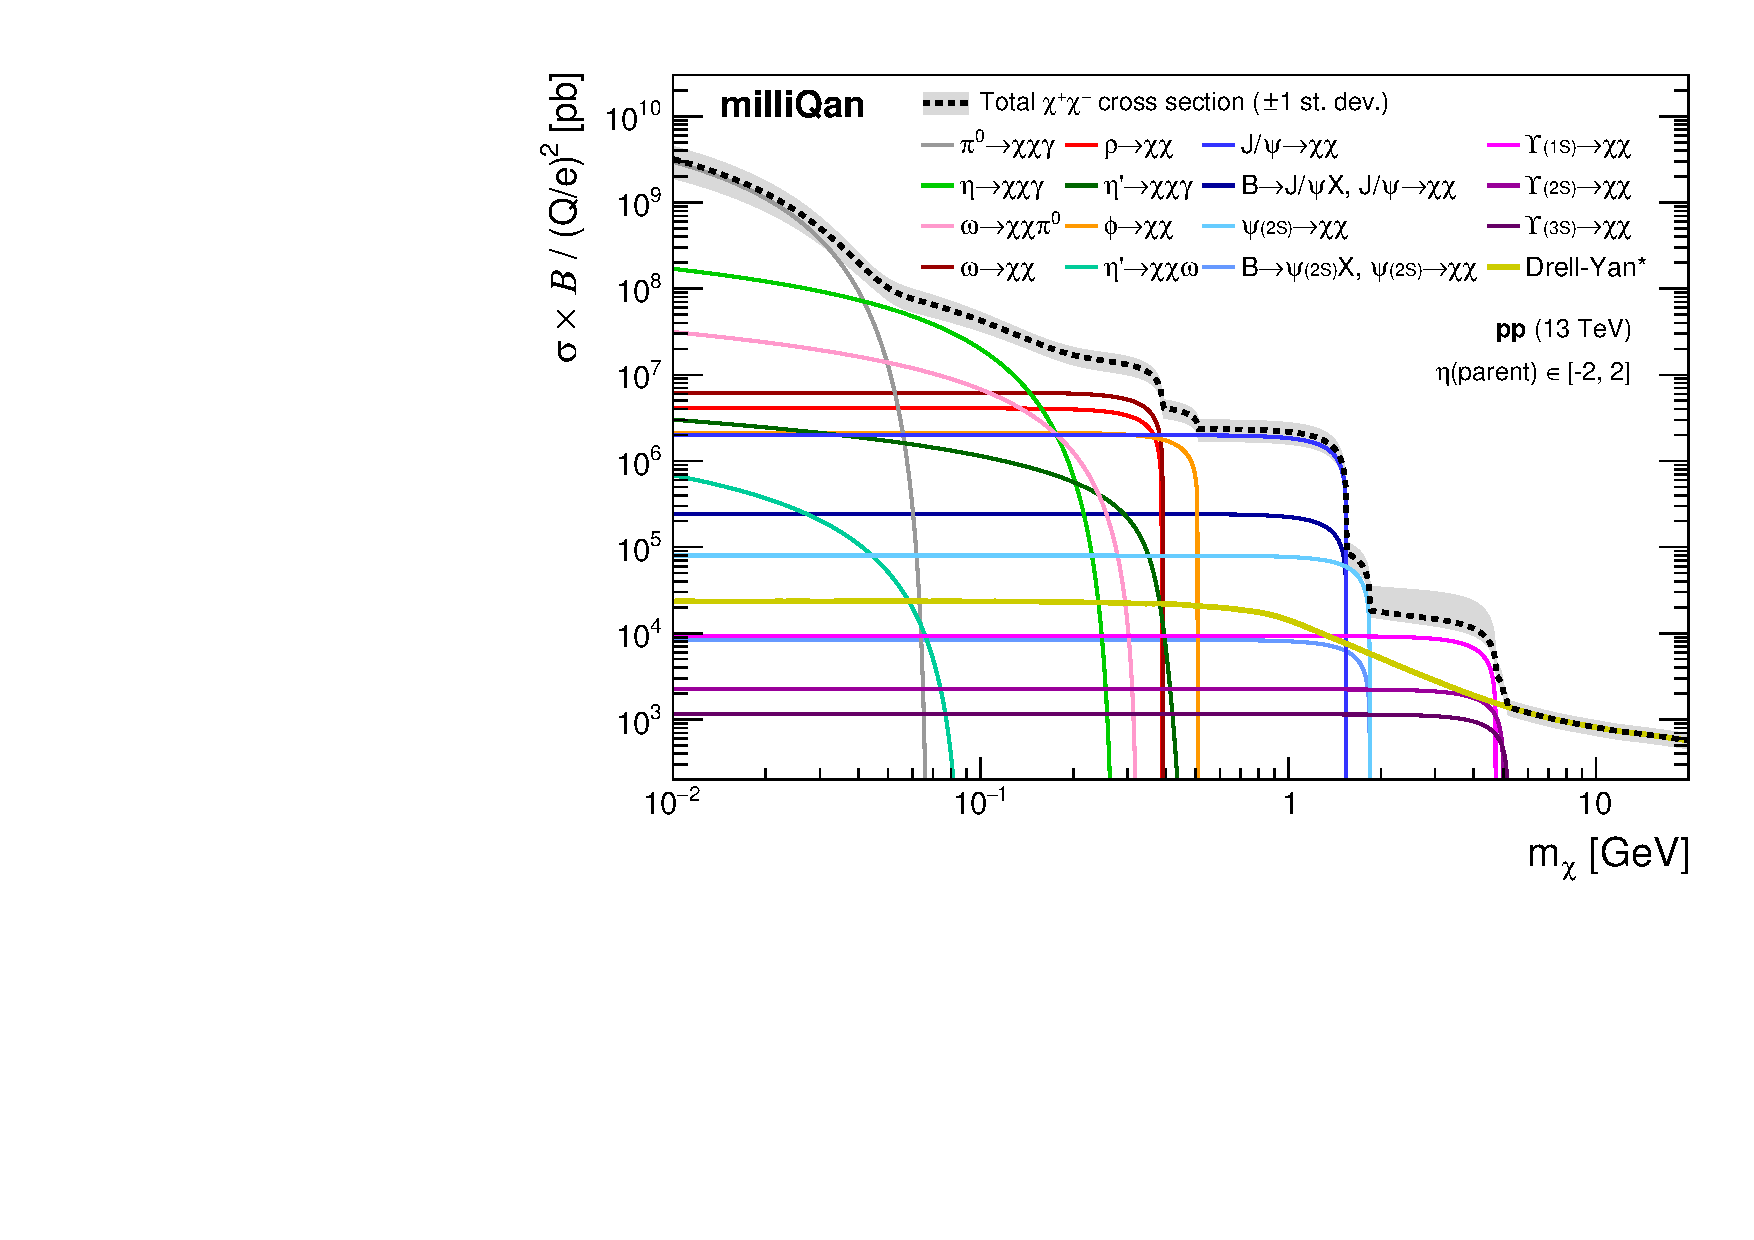
\includegraphics[width=0.80\textwidth]{figs/milliq/mcp-xsec.pdf}
    \caption{Cross section times branching ratio values for all considered
      production modes of $\zeta^+\zeta^-$ pairs, normalized to a charge
      of $Q/e=1$. For non-DY modes, the mother particle must be
      within $|\eta|<2$ (though the $\zeta^\pm$ may have $|\eta|>2$).
      For DY, the plotted cross section requires at least one mCP
      to have $|\eta|<1$. The plateau in DY cross section below 
      $m_\zeta=1\GeV$ is due to a 2\GeV $\zeta^+\zeta^-$ invariant
      mass cut in \textsc{Madgraph}. The gray band on the total
      cross section represents the total theoretical uncertainty
      in the cross section, adding in quadrature the uncertainties
      on each individual mode (with the exception of the 12.5\%
      $pp$ inelastic cross section uncertainty, which is correlated
      across all relevant modes).
            }
    \label{fig:mcp_xsec}
  \end{center}
\end{figure}

A plot summarizing the cross sectoin times branching ratio values
for all $\zeta^+\zeta^-$ production modes is shown in Fig.~\ref{fig:mcp_xsec}.
At low masses, production is dominated by Dalitz decays of light mesons
$\pi^0$, $\eta$. At around a few hundred \MeV, direct decays
of $\omega$'s and $\rho$'s dominate. Near 1\GeV, J/$\psi$'s provide
almost all of the cross section, before the rate falls off substantially
past half the J/$\psi$ mass near 1.5\GeV. $\Upsilon$'s become the dominant
production mode until they fall off at 5\GeV, after which
only Drell-Yan contributes. Note that if this plot were continued,
the rate would drop substantially again near half the $Z$ mass at
roughly 45\GeV.

Once all mCP four vectors are generated, they are propagated
through a model of the CMS and its environment, including
the magnetic field (see Fig.~\ref{fig:cms_bfield} for a colored map
of the magnetic field that is used), detector material, and 17 m of
rock between the IP and the drainage gallery.

The material geometry of CMS was extracted from a \textsc{Root} model,
and simplified into a series of concentric
iron cylinders, such that the total material budget is the same as that of the
real detector. Iron is placed at radii
\begin{itemize}\setlength\itemsep{-1mm}
\item $1.80 \leq r < 2.80$ m (tracker + HCAL)
\item $3.15 \leq r < 3.50$ m (magnet)
\item $3.85 \leq r < 4.05$ m (return yoke 1)
\item $4.60 \leq r < 4.95$ m (return yoke 2)
\item $5.35 \leq r < 5.95$ m (return yoke 3)
\item $6.35 \leq r < 7.15$ m (return yoke 4)
\end{itemize}

In addition to the iron, solid rock is placed at
$16 \leq r < 33$ m, until just before the face of the milliQan
detector.

Particles are propagated with a fourth-order Runge-Kutta
integrator, according to the relativistic kinematic equations
\be
\frac{d\vec{x}}{dt} = \vec{v} = \frac{\vec{p}c^2}{E} = \frac{\vec{p}c^2}{\sqrt{(\vec{p}c)^2+(mc^2)^2}}
\ee
\vspace{-6mm}
\be
\frac{d(\vec{p}c)}{dt} = 89.8755\;q\;\vec{v}\times\vec{B},
\ee
where the form of the second equation is valid if $B$ is in Tesla,
$t$ in ns, $\vec{v}$ in m/ns, $q$ in units of $e$, and $\vec{p}c$ in \MeV.

Multiple scattering is impolemented using a small-angle Gaussian angle approximation,
as described in the PDG~\cite{PDGreview33}. At each time step, a $\theta_\mrm{RMS}$ is 
computed based on the particle momentum and charge, the radiation length of the material,
and the distance traversed. Then two random deflection angles are drawn from a Gaussian of width
$\theta_\mrm{RMS}$, one for each transverse direction. The particle is also displaced
a small amount in the transverse plane, in a way that is partially correlated with the
angular deflection.

Finally, at each timestep the particle loses energy according to the Bethe equation
\be
\left\langle-\frac{dE}{dx}\right\rangle = Kz^2\frac{Z}{A}\frac{1}{\beta^2}\left[\frac{1}{2}\log\frac{2m_ec^2\beta^2\gamma^2W_\text{max}}{I^2} - \beta^2 - \frac{\delta(\beta\gamma)}{2} \right],
\ee{equation}
where all terms and parameters are defined in the PDG~\cite{PDGreview33}.
Note that energy loss is a stochastic process, and at each timestep the actual energy loss follows a highly skewed Landau distribution.
However, the amount of material traversed in this application is quite large, so it should be sufficient to use the mean value
at each timestep. At any rate, a systematic is assessed on the interaction with matter that should cover for any inaccuracies
in the modeling of energy loss.

Particles (either muons or mCPs) are propagated until 2 m before the face of the milliQan detector
after which they are fed into a full \textsc{Geant4}~\cite{geant4} simulation of the detector.
This includes a full model of the drainage gallery, aluminum support structure,
scintillator bars/slabs/panels with wrapping, lead bricks, and PMTs.
Quantum efficiencies of the simulated PMTs are set individually on a per-channel
basis so that the average number of PEs generated by a cosmic and/or beam 
muon match that measured data, from the calibrations described in 
Sec.~\ref{sec:insitu_calib}. An illustration of a beam-based muon
traveling through the \textsc{Geant} model of the detector is 
shown in Fig.~\ref{fig:mq_geant}.

\begin{figure}[t]
  \begin{center}
    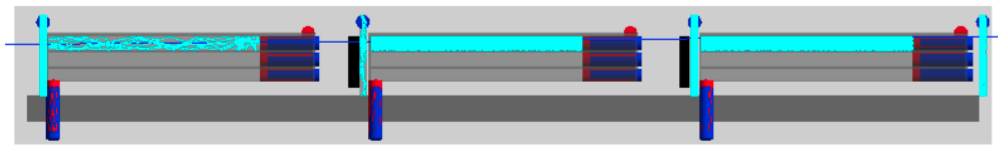
\includegraphics[width=0.750\textwidth]{figs/milliq/geant.png}
    \caption{Rendering of a beam-based muon traveling through
      a \textsc{Geant4} model of the demonstrator, hitting all
      four slabs and three bars in a straight line. Light blue
      lines are generated optical photons.
            }
    \label{fig:mq_geant}
  \end{center}
\end{figure}

The exact time of each detected photoelectron is saved, so that the \textsc{Geant} output
events can be used for \textit{pulse injection}, in which simulated PMT waveforms
are overlaid on zero-bias (i.e. random trigger) data, in order to generate realistic
detector signals that can be processed and analyzed with the same software as real data.
For each simulated PE, a random SPE area is drawn from PMT-specific
distributions dervied via PMT bench tests, described in Sec.~\ref{sec:pmt_bench_tests}
(these distributions are corrected for slight differences between channels).
Then a template SPE waveform, also derived from the PMT bench tests, is scaled to this
area and overlaid on a random zero-bias event. These pulse-injected simulated events
then look just like real data, with the exception that they do not model
PMT saturation effects (however, this does not matter in practice).

\section{Simulation validation and data comparisons}


\section{Background estimation and results}


}

